\documentclass{article}
\usepackage[a4paper, total={6in, 10in}]{geometry}
\setlength{\parskip}{0.01cm plus4mm minus3mm}

\usepackage{multicol}
\usepackage{enumitem}

\usepackage{listings}
\usepackage{xparse}

\usepackage[superscript,biblabel]{cite}
\usepackage{graphicx}
\usepackage{hyperref}
\usepackage{caption}

\usepackage{xcolor}
\colorlet{cBlue}{blue!80}
\colorlet{cPurple}{blue!40!red}

\NewDocumentCommand{\codeword}{v}{
    \texttt{\textcolor{cBlue}{#1}}
}

\NewDocumentCommand{\cmd}{v}{
    \textit{\textcolor{cPurple}{#1}}
}

\title{World of Deez}
\author{Pawel Makles \\ \small (K21002534)}
\date{\small Created: 19th November 2021 \\ Last Modified: 3rd December 2021}

\begin{document}
\maketitle

    \begin{multicols}{2}
        \section{User Level Description}
        This game is largely open world but has a main storyline which the player can choose to follow to complete the game, as well as other side-quests which can be done alongside or after the story.

        In this game, you are one of millions of citizens in an isolated city home to a Beastman \cite{beastman} society, the city being loosely based off Animacity \cite{animacity} from the series Brand New Animal \cite{bna}. The plot revolves Sylvasta who are deeply intertwined with the city and own the city's medical centre.

        There have been reports that their research has been highly unethical and leaks have been coming out from former employees which have been riling up protests throughout the city, your goal is to figure out what's really happening and to put a stop to it.

        I ended up not adding any information about the main character as to add to the open world, `your adventure', feeling. The story is also loosely based off Utopia \cite{utopia}, in which a group of people are finding the truth behind a manuscript and find themselves in the middle of a conspiracy \cite{pyrocynical}.
        
        \section{Implementation}
        The project is split up into several packages, most of which work independently of each other, in general, the \codeword{Game} uses the \codeword{commands} package (providing actions the player can perform) along with the \codeword{world} (providing the things that the player can interact with in the game) package to run the game. They are laid out as follows:
        
            \subsection{Commands}
            This package provides the classes required to parse and run commands, it includes the \codeword{CommandManager} which registers objects of type \codeword{Command}. More about parsing commands is in the challenge task section.

            This package also includes a subpackage called \codeword{core} containing all of the `core' commands required to run any game world, this includes things such as picking items up, quiting the game, and so forth.
            
            \subsection{Entities}
            This package provides the basic tools required to create simple and complex entities within the world, more about entity detail is discussed later.

            It also contains a subpackage \codeword{actions} which contains common interfaces which entities can implement to allow the ways that they can be interacted with to be quite modular.
            
            \subsection{Content / Campaign}
            The \codeword{content.campaign} package contains a lot of custom content derived from the base game used to construct the story and the story world.
            
            \subsection{World}
            This package has the basic building blocks for creating worlds including the \codeword{World} and \codeword{Room} classes which can be easily extended for more functionality. The only limitations are that traveling between rooms must be done in a direction specified in the \codeword{Direction} enum and that the \codeword{Location} of any entity must be either a room, inventory or neither.
            
            \subsection{Util}
            This package contains a bunch of small utility classes, including:

                \begin{itemize}[leftmargin=*]
                    \item \textbf{BlueJ.java} \cite{bluej}: Contains improved methods on detecting whether the application is currently running in BlueJ. (taken from my previous coursework assignment)
                    \item \textbf{Localisation.java}: A pretty straightforward implementation of a localisation engine. Simply maps (period-separated) keys to their respective (nested) keys in a language file.
                    \item \textbf{Search.java}: Methods for searching through various data structures in the game.
                    \item \textbf{Tree.java}: A very simple implementation of a tree with basic traversal methods.
                \end{itemize}

            \subsection{Dialogue \& IO \& UI \& Events}
            These are all discussed later on in the challenge task section.

        \section{Base Tasks}

            This section describes how I implemented the basic task requirements.

            \begin{itemize}[leftmargin=*]
                \item \textit{``The game has several locations the player can walk through.''}
                
                    I began by first designing the world map (see \autoref{fig:map}), using Excalidraw \cite{excalidraw}, then implemented each location as a \codeword{Room}.

                    To build the world, I made a \codeword{World} class to house all the locations which exist in the game world and then extended this using the \codeword{CampaignWorld} class which builds the story world, creates rooms and registers events.

                    I ended up adding $10$ locations into my game:
                    \begin{itemize}[leftmargin=*]
                        \item \textbf{City Centre}: Centre of the city connecting major areas with the coast.
                        \item \textbf{Apartments}: This is the player's residence.
                        \item \textbf{Street}: This is the main city street connecting important buildings.
                        \item \textbf{Shop}: The local city shop where the player frequents to get necessary items.
                        \item \textbf{Back Alley}: This is where the player can start the main story mission.
                        \item \textbf{Coastline}: There are two coasts, one on the city side and one on the mainland.
                        \item \textbf{Forest}: The forest grants access to the Worm Hole and to other side-quests.
                        \item \textbf{Worm Hole}: For challenge task 3.
                    \end{itemize}

                    The layout is heavily inspired by Animacity, although since there's no available map of the actual city, I made my own interpretation based off various pieces of art, (see \autoref{fig:runaway-raccoon}). I used an existing real life location to determine the size of the river \cite{river-map}.

                \item \textit{``There are items in some rooms that may or may not be picked up by players.''}
                
                    To achieve this, I considered all entities to be items which may or may not be picked up by other entities, each entity has its own \codeword{Inventory} which is in effect a list of other entities which it is holding.
                
                \item \textit{``Each item has a weight and the player can only carry items up to a certain weight.''}
                
                    To do this, I added a new private field \codeword{weight} of type double to the \codeword{Entity} class, which is used to store the entity's weight. It is a double as I wanted access to fractional weights (say $0.01$kg) and I wanted to have access to \codeword{Stream::mapToDouble} for summations.

                    For the second part, I made it so each \codeword{Inventory} has a maximum weight it can store, which by default is set to $0$ as each entity has an inventory but may not necessarily have the ability to store anything.

                    When putting anything in an inventory, we check that the following is satisfied:
                    $$
                        \textsf{currentWeight} + \textsf{itemWeight} \le \textsf{maxWeight}
                    $$

                    To determine the weight of common items, I referred to a document I found online published by the City of York Council \cite{common-weights}.
                
                \item \textit{``Player can win.''}
                
                    The player may win by completing the main story mission (detailed in the walkthrough) which sets a flag that the game has been completed, the player may choose to keep playing in the open world or run \cmd{win} to end the game.

                \item \textit{``There is a command} \cmd{back} {which takes you back to the last room.''}
                
                    I added two new private fields to the player entity, which were \codeword{previousRooms} and \codeword{retreatingDirection}, these are used to store the path back through the room and the direction which we need to go to get back there respectively. The direction is stored in order to run a check whether the player can actually go back in the direction they intend to, to verify this, the `retreating direction' is used to call the method \codeword{canLeave} on the current room the player is in.

                \item \textit{``Add at least four new commands.''}
                
                    I added several additional commands which are listed below:

                    \begin{itemize}[leftmargin=*]
                        \item \cmd{bag}: Allows the player to look at their or another entity's inventory.
                        \item \cmd{drop}: Drop any specified item from the player's inventory into current room.
                        \item \cmd{give}: Give a specified item to another entity, we ensure that the entity implements \codeword{IGiveable} and give the item to the entity using \codeword{IGiveable::give}.
                        \item \cmd{pet}: Pet a specified entity, has to implement \codeword{IPettable}, we use \codeword{IPettable::pet}.
                        \item \cmd{take}: Take any specified item from another entity's inventory.
                        \item \cmd{talk}: Initiate a conversation with an entity, must implement \codeword{ITalkwith}, we call \codeword{ITalkwith::talk} to start the conversation.
                        \item \cmd{use}: `Use' an entity, we call \codeword{IUseable::use} to use the entity. (implemented by entity)
                        \item \cmd{where am i}: Tells the game to print out room information again, this is done by emitting \codeword{EventEntityEnteredRoom} again.
                    \end{itemize}

                    See \autoref{fig:help-command} for an example of the help menu.
            \end{itemize}

        \section{Challenge Tasks}

            This section describes how I implemented the challenge tasks and what I did in addition.

            \subsection{Required Tasks}
            \begin{itemize}[leftmargin=*]
                \item \textit{``Add characters to your game.''}
                
                    %

                \item \textit{``Extend the parser.''}
                
                    I entirely replaced how the parser worked, I began by implementing a basic model of \codeword{Command}, it took a few iterations but I settled on providing Regex \codeword{Pattern}s.

                    This approach has several benefits:

                    \begin{itemize}[leftmargin=*]
                        \item Powerful Regex at low performance cost due to the low number of commands.
                        \item Ability to have named capture groups which are then interpreted as arguments.
                    \end{itemize}

                    For each known \codeword{Command}, I would create a \codeword{Matcher} for each \codeword{Pattern}, execute it against the arbitrary command from the user and then pass it into a wrapper class \codeword{Arguments} which lets me safely pull out named groups, directions or any other argument type I need.
                
                \item \textit{``Add a magic transporter room.''}
                
                    To do this, I added a \codeword{RoomWormHole} which I made implement \codeword{EventEntityEnteredRoom} to listen for when any entities entered the room, as soon as one is detected, a short animation is played and a room is selected at random to teleport the user to. Allowing the user to go to \textbf{any room} may interfere with my story so I chose to only spawn the user at any outside areas of the map.
            \end{itemize}

            \subsection{Dialogue and Localisation}
            \textit{``Give NPCs interactive dynamic dialogue.''}

            \subsection{World Event System}
            \textit{``Add a system for managing world events.''}

            \subsection{Terminal Emulator}
            \textit{``Implement a terminal emulator.''}

            I implemented this by creating a new class \codeword{TerminalEmulator} which implements the \codeword{IOSystem} so that it could be easily slotted into the game. 

            \subsubsection{Ansi Escape Codes}
            \subsubsection{Emoji Support}
            \subsubsection{EventDraw and the Map}

        \section{Code Quality}
        % For each of the following code quality considerations, give and explain an example in your
        % project where you considered it: coupling, cohesion, responsibility-driven design, maintain-
        % ability.

        \section{Walkthrough}
        %

        \section{Known Issues}
        
            \begin{itemize}[leftmargin=*]
                \item find issue
            \end{itemize}

    \end{multicols}

    \newpage

    \begin{thebibliography}{9}
        \bibitem{beastman}
        Brand New Animal Wiki. Beastman \url{https://brand-new-animal.fandom.com/wiki/Beastman}
        \bibitem{animacity}
        Brand New Animal Wiki. Animacity \url{https://brand-new-animal.fandom.com/wiki/Anima_City}
        \bibitem{bna}
        IMDb. BNA (TV Mini Series 2020) \url{https://www.imdb.com/title/tt12013558/}
        \bibitem{utopia}
        IMDb. Utopia (TV Series 2013-2014) \url{https://www.imdb.com/title/tt2384811/}
        \bibitem{excalidraw}
        Excalidraw. \url{https://excalidraw.com/}
        \bibitem{bluej}
        GitHub. maven-bluej / BlueJ.java \url{https://github.com/KCLOSS/maven-bluej/blob/master/BlueJ.java}
        \bibitem{river-map}
        Google Maps. Jezioro Świerklaniec, Poland \url{https://www.google.com/maps/@50.4293559,18.9742453,16.12z}
        \bibitem{common-weights}
        PDF. Set of average weights for furniture, appliances and other items \url{https://democracy.york.gov.uk/documents/s2116/Annex\%20C\%20REcycling\%20Report\%20frnweights2005.pdf}
        \bibitem{pyrocynical}
        YouTube. The best (and worst) show you haven't seen \url{https://youtu.be/PFx2QM0Z8Qo}
    \end{thebibliography}  
    
    \newpage

    % Appendix
    \captionsetup{justification=centering,margin=3cm}
    \begin{figure}
        \centering
        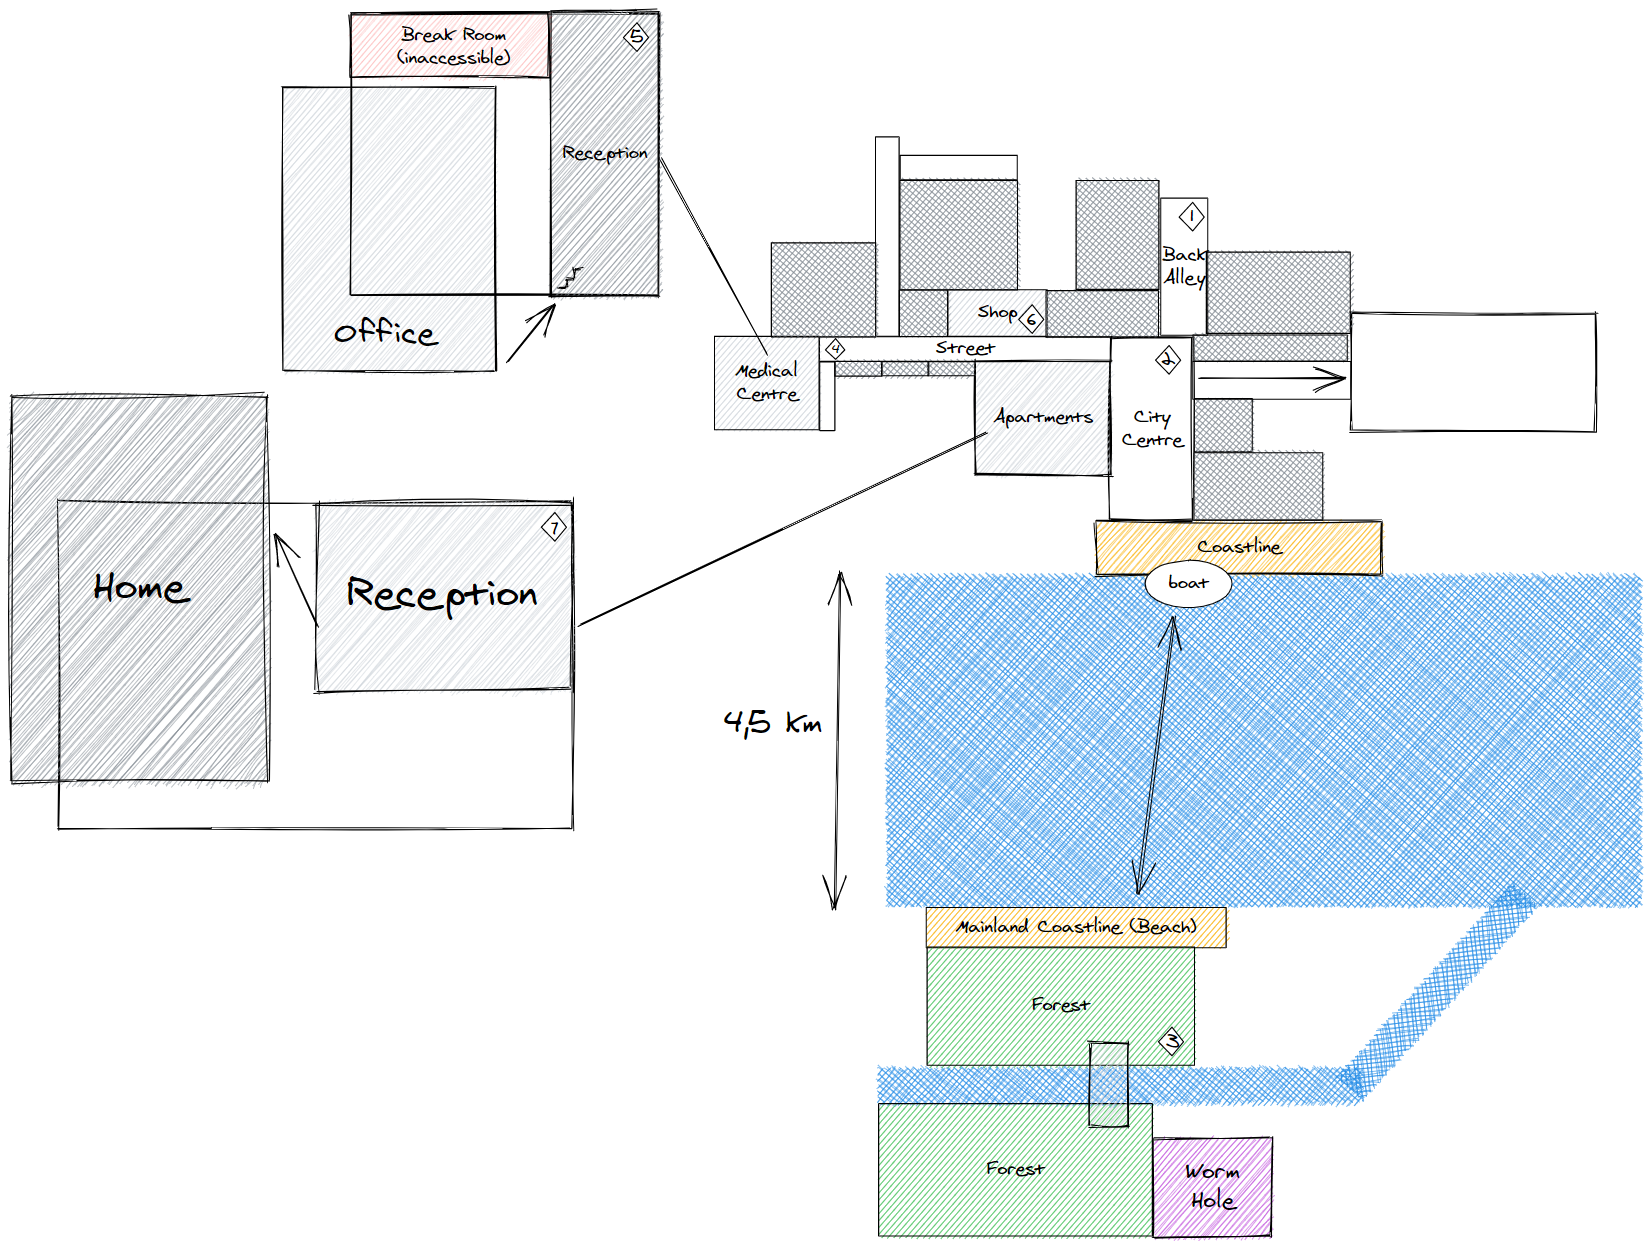
\includegraphics[width=\textwidth]{../src/main/resources/map/base.png}
        \caption{World Map} \label{fig:map}
    \end{figure}
    \begin{figure}
        \centering
        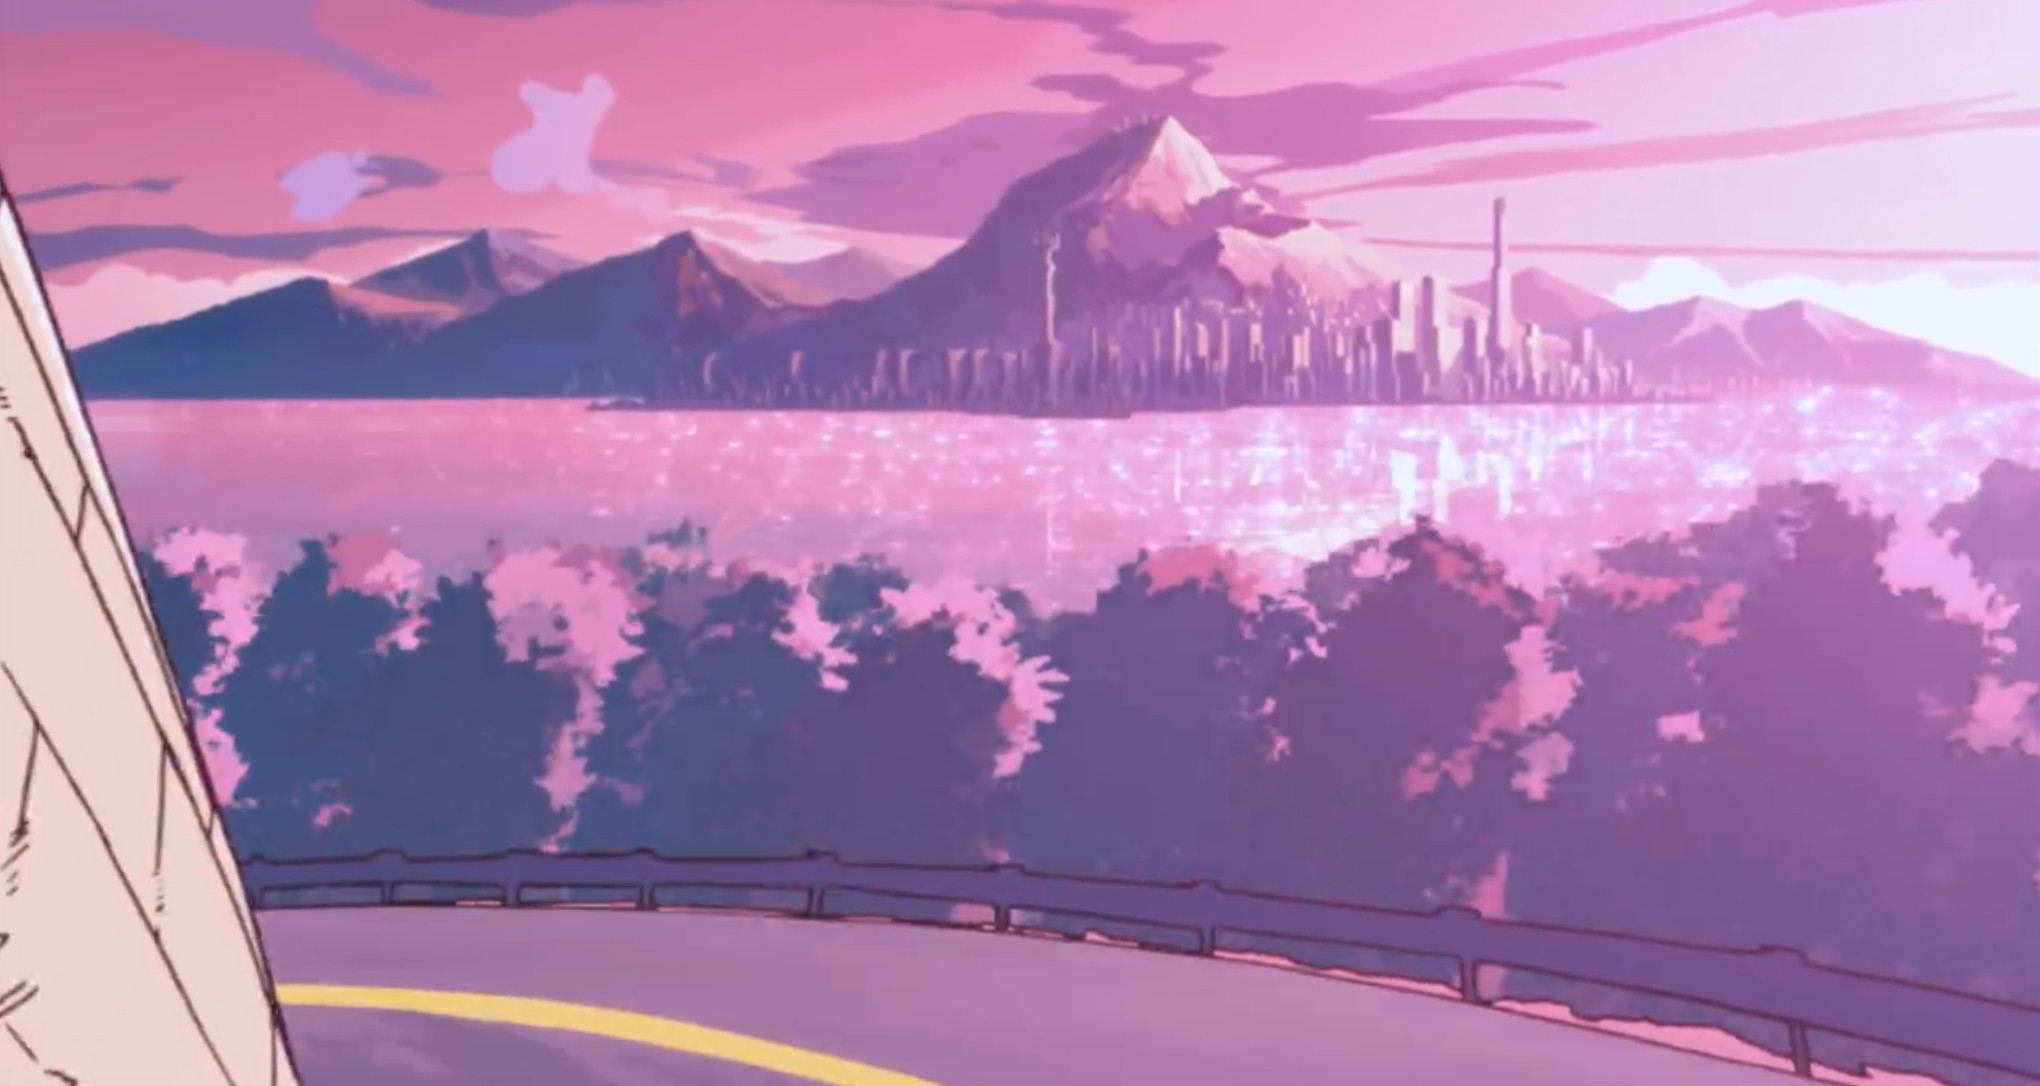
\includegraphics[width=\textwidth]{images/runaway-raccoon-302.jpg}
        \caption{Shot of Animacity as seen in Episode 1 at 3:02 of Brand New Animal \cite{bna}} \label{fig:runaway-raccoon}
    \end{figure}
    \begin{figure}
        \centering
        
\includegraphics[width=\textwidth]{images/festival-marie.jpg}
        \caption{Michiru Kagemori and Marie Itami pictured left to right in Episode 1 at 12:51 of Brand New Animal \cite{bna}} \label{fig:festival-marie}
    \end{figure}
    \begin{figure}
        \centering
        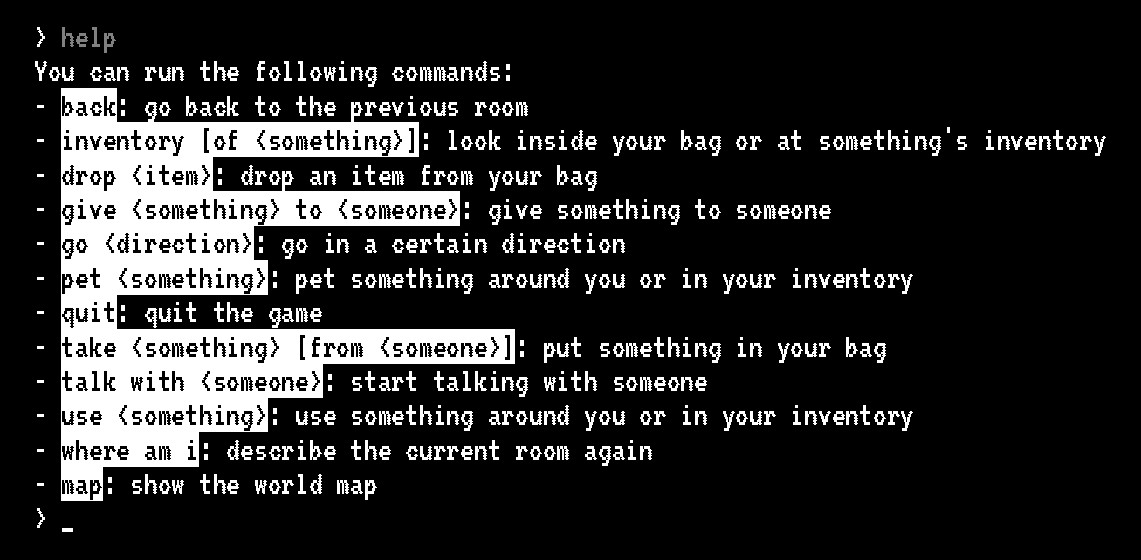
\includegraphics[width=\textwidth]{images/help-command.jpg}
        \caption{Output from the help command} \label{fig:help-command}
    \end{figure}
\end{document}
